\IEEEraisesectionheading{\section{简介}
\label{sec:introduction}}

超分辨率重建指的是将给定的低分辨率图像恢复成相应的高分辨率图像,单图超分旨在利用空间信息将给定的低分辨率图像恢复成相应的高分辨率图像,而对于视频来讲,多帧高度相关但不对齐的图像可以为超分提供更加丰富的信息,对这些帧间信息的利用是几乎所有视频恢复任务比较核心的研究课题。

如 \textbf{图 \ref{fig:fig2}} 所示,可以看到对孔洞进行恢复时,单图超分由于难以获得语义信息,所以恢复得不太准确,而视频超分由于综合了多帧的信息,可以恢复出更加准确的细节。而在日常拍照时,快门按下去并不一定是一帧被采集,而是会连续采集很多帧,帧之间微小的抖动可以提供了很多视频恢复使用的亚像素信息。


上面一排是相同的但有微小位移的高分辨率图片,下面是对应的低分辨率版本。虽然都占据了相同的像素,但是当高分辨率的图像位移1/4或者1/2个像素的时候,产生的低分辨率的版本是不同的,由位移产生的这些不同模式就是所说的亚像素的信息。

上面一排是有微小位移的相同高分辨率图片,下面是对应的低分辨率版本。虽然都占据了相同的像素,但是当高分辨率图像位移1/4或者1/2个像素的时候,产生的低分辨率的版本是不同的,由位移产生的这些不同模式就是所说的亚像素的信息。

对于单图和视频超分,一个朴素的做法就是使用相同的超分网络,单图把所有的空间信息交给网络去预测,对于视频可以把帧间的信息叠在一起之后交给网络预测。但有一个问题就是视频里面的物体是会移动的,而由于 CNN 具有局部性的归纳偏置,这显然是行不通的。因此需要对网络进行一些特殊的模块设计。

\begin{figure}[!tbp]
	\centering
	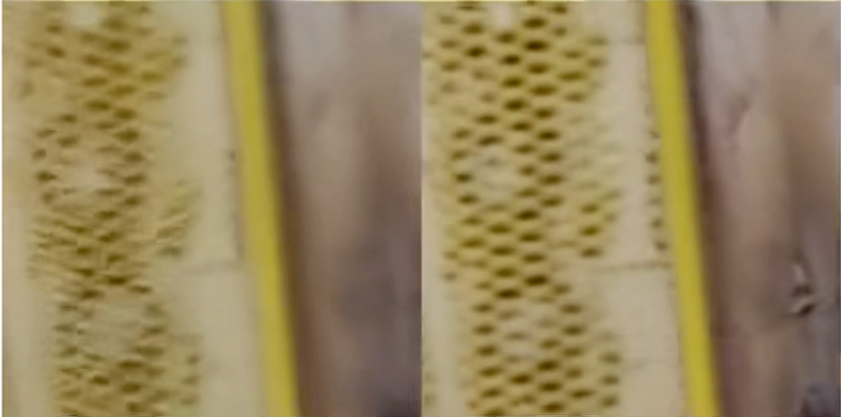
\includegraphics[width=0.9\linewidth]{3.png}
	\caption{SISR 和 VSR 模型的视频超分辨率重建结果:左:SISR, 右:VSR}
	\label{fig:fig2}
\end{figure}